\section{Related Works}

We focus on structure-preserving, deployable navigation with deformable bodies under strict local sensing. Our work intersects geometric and Hamiltonian learning, safety-critical control, deformable robot navigation, neural scene representations, and simultaneous navigation and mapping.

\paragraph{Geometric Reinforcement Learning in navigation.}
Most navigation RL methods treat the problem as control in flat Euclidean spaces using standard algorithms such as PPO and TD3~\citep{schulman2017ppo,fujimoto2018td3}. Variants with richer reward shaping or auxiliary losses improve collision avoidance~\citep{taheri2024enhanced}, but still ignore the underlying geometric structure and typically require millions of interactions for robust performance~\citep{dehghani2024survey}. Geometric approaches explicitly exploit configuration-space structure: SE(2)/SE(3)-equivariant policies for manipulation~\citep{hoang2025geometry}, Riemannian formulations that enforce constraints via tangent-space projections~\citep{martinez2023accelerated, riemannian2023safe}, and Hamiltonian / port-Hamiltonian neural networks that preserve symplectic structure and energy~\citep{aps2021port}. However, these works are largely restricted to simple control or manipulation tasks, do not address deformable-body navigation, and are not designed for SNAM. In contrast, GRL-SNAM uses a Hamiltonian formulation for \emph{navigation itself}: sensing, path planning, and deformation all evolve on a shared energy manifold with differential policy optimization rather than ad-hoc Euclidean policy updates. 

We consider the geometric property in the RL policy iteration itself as well. Most mainstream deep RL algorithms are developed within the dynamic programming principle (DPP): they optimize either value functions or policy surrogates whose correctness is ultimately justified by Bellman consistency. This includes value-based and actor–critic families, even when the update is implemented via policy gradients (e.g., PPO, SAC, TRPO), because the critic and advantage estimates are derived from Bellman-style recursions rather than from Hamilton–Jacobi–Bellman (HJB) analysis or dual optimal control constructions. In contrast, our approach follows a growing line of work that explicitly departs from DPP and instead leverages continuous-time optimal control structure—HJB and/or duality-based Hamiltonian formulations—to define learning objectives and updates without relying on Bellman backups. Representative examples include model-free HJB-based learning \citep{settai2025temporal}, martingale formulations that reinterpret or relax DPP conditions \citep{jia2023qlearning}, and duality-driven Hamiltonian RL \citep{dpo}, which we build upon and extend. The key distinction between GRL-SNAM and other RL navigation methods is two-folded: we do not reparameterize value-function gradients; we learn and adapt a reduced Hamiltonian whose energy decomposition directly induces the closed-loop dynamics. We refer readers Figure \ref{fig:rl_comparison} for a comparison statement.

\begin{figure}[!htbp]
\centering
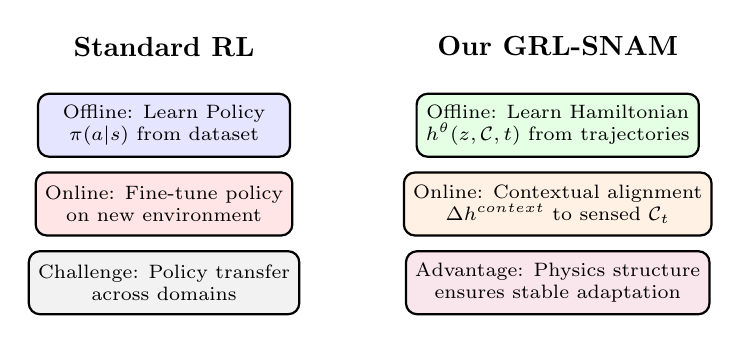
\begin{tikzpicture}[
    node distance=0.8cm,
    box/.style={rectangle,draw,thick,rounded corners,minimum width=3.2cm,minimum height=0.8cm,align=center,font=\scriptsize},
    approach/.style={font=\bfseries},
]

% Standard RL Approach
\node[approach] at (-4,3.5) {Standard RL};
\node[box,fill=blue!10] at (-4,2.5) {Offline: Learn Policy\\$\pi(a|s)$ from dataset};
\node[box,fill=red!10] at (-4,1.5) {Online: Fine-tune policy\\on new environment};
\node[box,fill=gray!10] at (-4,0.5) {Challenge: Policy transfer\\across domains};

% Our GRL-SNAM Approach
\node[approach] at (1,3.5) {Our GRL-SNAM};
\node[box,fill=green!10] at (1,2.5) {Offline: Learn Hamiltonian\\$h^{\theta}(z,\mathcal{C},t)$ from trajectories};
\node[box,fill=orange!10] at (1,1.5) {Online: Contextual alignment\\$\Delta h^{\text{context}}$ to sensed $\mathcal{C}_t$};
\node[box,fill=purple!10] at (1,0.5) {Advantage: Physics structure\\ensures stable adaptation};

\end{tikzpicture}
\caption{Comparison between standard RL offline/online adaptation and our physics-grounded approach. Standard methods learn arbitrary policies and struggle with transfer, while our approach learns physically meaningful Hamiltonians that naturally adapt to environmental variations.}
\label{fig:rl_comparison}
\end{figure}



\paragraph{Safety-critical and reward-exploring navigation.}

When training to plan obstacle-avoidance paths, the design of reward affects the quality of output trajectories via policy learning. Earlier work focuses on handcrafted or intrinsic curiosity reward \citep{tai2017virtual, Lei2018curiosity}. Control Barrier Functions (CBFs) have emerged as a principled way to enforce safety by projecting candidate actions into a safe set, including model-based CBF-RL combinations~\citep{li2023imagination}, neural zeroing barrier functions~\citep{feng2023safer}, adaptive barrier mechanisms for dynamic environments~\citep{sac2025barrier}, and social-navigation CBFs for human--robot interaction~\citep{social2024barrier}. While these methods provide formal safety guarantees, safety is typically treated as an \emph{external projection layer} on top of an otherwise standard controller, which often leads to conservative, sometimes myopic behavior and weak coupling between task optimality and safety. GRL-SNAM instead integrates safety \emph{within} the Hamiltonian energy via barrier potentials: obstacles, free-space preferences, and goal attraction jointly shape the local energy landscape, so that safety and optimality are co-optimized under a symplectic, structure-preserving flow.

\paragraph{Deformable and soft robot navigation.}
Soft and deformable robots have motivated sophisticated modeling and control techniques, including hyperelastic material models with pressure-stiffening control~\citep{roshanfar2023hyperelastic}, passivity-based control via differential geometry of curves~\citep{caasenbrood2022control}, and spectral submanifold reduction for real-time hyperelastic control~\citep{nature2025discovering}. Physics-informed learning further improves fidelity: PINN-Ray~\citep{wang2024pinn} and related models for non-conservative effects~\citep{liu2024physics} achieve accurate displacement prediction but primarily target offline modeling rather than adaptive navigation. For navigation specifically, ring-like or morphable bodies such as aerial LCE-based gap navigators~\citep{qi2024aerial} and HAVEN~\citep{haven2024haptic} use pre-programmed deformation sequences or offline-optimized actuation patterns with deterministic execution. These systems cannot adapt deformation strategies online when geometry of environment changes, and they lack a unifying energy-based view that couples shape, motion, and sensing. GRL-SNAM fills this gap by treating the deformable robot as an energy-carrying body: deformation penalties, contact forces, and path costs are encoded in a Hamiltonian whose gradients drive both motion and shape control under changing local observations.

\paragraph{Neural scene representations for navigation.}
Neural implicit maps provide dense geometric information for navigation. NeRF-based SLAM methods such as NICE-SLAM~\citep{zhu2022nice} and iMAP~\citep{sucar2021imap} reconstruct detailed 3D scenes, while Neural Topological SLAM~\citep{chaplot2020neural} and semantic extensions with large vision models~\citep{zheng2025semantic} combine learned mapping with classical planning. 3D Gaussian splatting approaches like GS-SLAM~\citep{yan2024gs} and SplaTAM~\citep{keetha2024splatam} offer real-time, high-fidelity reconstruction suitable for robot navigation. These methods aim to build accurate maps; the control policy is typically a separate planning layer, and the system often assumes the luxury of extensive mapping before or during navigation. GRL-SNAM is complementary: any of these scene representations can be converted into signed-distance and occupancy-derived potentials for our barrier and goal terms, but our objective is to \emph{minimize mapping effort}, using only local observations to progressively refine a Hamiltonian that encodes the task.

\paragraph{Simultaneous navigation and mapping (SNAM).}
Most SNAM methods prioritize constructing rich global maps and then planning on them. SGoLAM~\citep{sgolam2021} couples goal localization with occupancy mapping, CMP~\citep{gupta2017cognitive} integrates a differentiable planner into a learned map, and CL-SLAM~\citep{clslam2022} focuses on maintaining maps for long-term operation. These approaches do not explicitly reason about the cost of mapping itself and are not designed for deformable bodies or binded with optimal control problems. Some works encourage to learn a context-aware reward \citep{liang2023context} or an explicit terrain cost map \citep{sathyamoorthy2022terrapn} that can be used to compute dynamically feasible trajectories while simultaneously reading the partial map, yet they still rely on RL-driven policy network or model-based fixed rule (i.e. DWA, \citet{fox2002dynamic}) to apply the learned reward/cost. GRL-SNAM instead targets \emph{joint exploration}: the robot maintains only the local information needed to define a good energy landscape around its current belief, continually refining least-cost trajectories as new observations arrive rather than insisting on globally complete maps.

\paragraph{Hierarchical, multi-agent, and imitation-based navigation.}
Hierarchical RL decomposes complex navigation into sub-tasks with high-level coordinators, as in HRL4IN~\citep{li2020hrl4in} and adaptive policy-family methods~\citep{lee2023adaptive}. Multi-agent frameworks such as RoboBallet~\citep{lai2025roboballet} and MACRPO~\citep{macrpo2024} achieve impressive coordinated behavior using graph-based policies and improved information sharing. However, these methods typically rely on manually specified hierarchies or reward structures and seldom preserve underlying geometric or energy structure, making it difficult to guarantee stable coordination across time scales. Imitation learning and inverse RL further improve sample efficiency using expert trajectories: large-scale behavioral cloning (RT-1)~\citep{brohan2022rt1}, safe imitation via GAIL-style methods~\citep{gail2024safe}, DAgger-based continuous navigation~\citep{shi2025dagger}, and confidence-aware imitation for sub-optimal demonstrations~\citep{confident2024il}. These approaches are powerful when high-quality demonstrations exist but struggle when expert coverage of the full deformation and contact behavior space is limited. GRL-SNAM shares with hierarchical and imitation methods the aim of efficient learning but differs in \emph{how} structure is encoded: we do not hand-design a task graph; instead, sensing, path, and deformation policies are coupled through a shared Hamiltonian with differential updates, yielding principled multi-scale coordination and stability guarantees.

\paragraph{Foundation models for navigation reasoning.}
Recent work leverages large foundation models for high-level navigation reasoning, goal inference, and multi-agent coordination~\citep{zhu2024navi2gazeleveragingfoundationmodels,llm2025nav}. These systems excel at semantic understanding, language-grounded objectives, and flexible decision-making but generally outsource low-level control to conventional planners or RL policies, creating a gap between symbolic reasoning and physically consistent motion. GRL-SNAM is complementary: foundation models can supply high-level instructions or semantic goals that we encode as potential energy terms in our Hamiltonian, while our structure-preserving dynamics ensure that these goals translate into safe, physically plausible trajectories for a deformable body under local sensing.

\paragraph{Positioning of GRL-SNAM.}
Across these paradigms, existing methods typically provide \emph{some} of: geometric structure, safety, sample efficiency, deformable-body support, or SNAM capabilities, but not all simultaneously. Our GRL-SNAM framework is, to our knowledge, the first to (i) formulate deformable-body SNAM as coupled Hamiltonian dynamics on a shared energy manifold under strict local sensing, (ii) integrate safety, deformation costs, and navigation objectives directly into the energy rather than in external projection layers, and (iii) coordinate sensing, planning, and deformation via a differential multi-policy architecture with symplectic updates. This combination yields high-quality, well-weighted paths with minimal mapping effort, while preserving geometric structure and enabling principled analysis of stability and convergence.